

\subsection{Introducción}

En este trabajo practico trabajaremos con procesamiento de imagenes. Implementaremos dos filtros, blur y diff, ambos en dos lenguajes diferentes, assembler y c. \\


El diff, o diferencia de imagenes, toma como parametro dos imagenes y generara una nueva en la que se resalta donde difieren, en escala de grises. Para cada par de pixeles correspondientes, se calcula la maxima diferencia entre sus componentes y la misma se devuelve en el pixel correspondiente de la imagen de salida \\


\begin{figure}[H]
\begin{center}

\minipage{0.5\textwidth}
  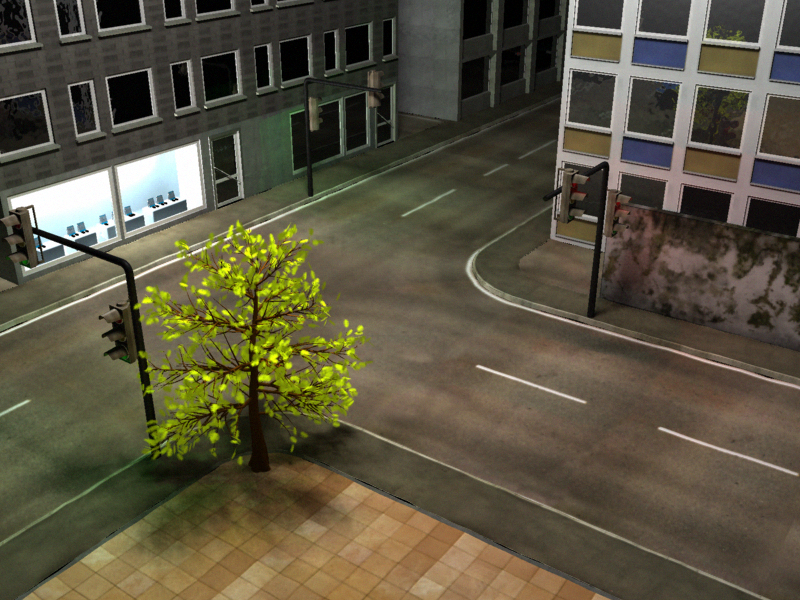
\includegraphics[width=\linewidth]{img/scene0(1).png}
  \caption{{\small Imagen 1}} 
\endminipage
\minipage{0.5\textwidth}
  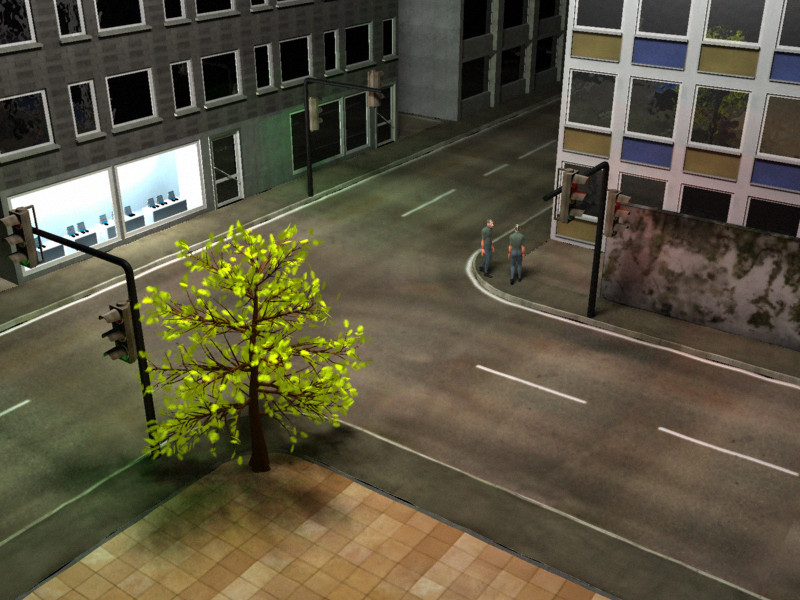
\includegraphics[width=\linewidth]{img/scene400.png}
  \caption{{\small Imagen 2}} 
\endminipage

\end{center}
\end{figure}

\begin{figure}[H]
\begin{center}

\minipage{0.6\textwidth}
  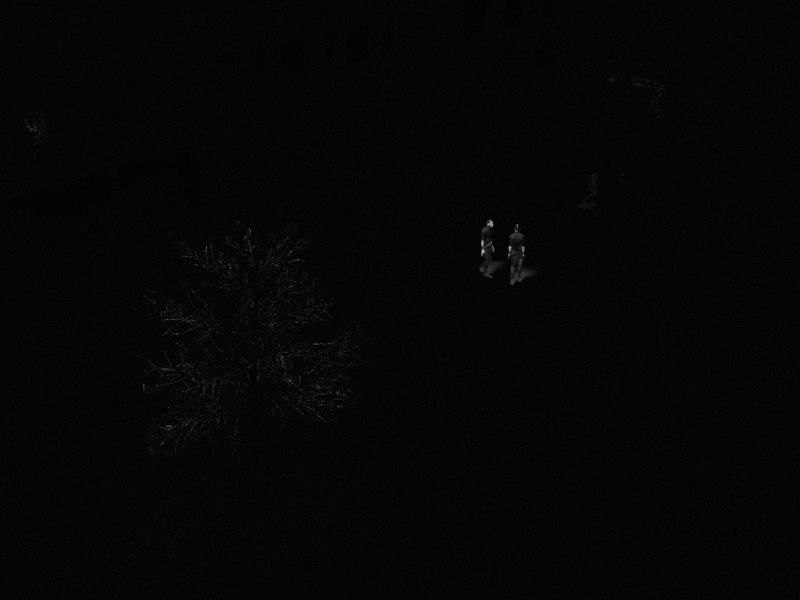
\includegraphics[width=\linewidth]{img/scene0.png}
  \caption{{\small Resultado}} 
\endminipage

\end{center}
\end{figure}

El blur (gaussiano) consiste en un suavizado de la imagen, para darle un aspecto desenfocado a la misma. El mismo toma como parametro una imagen, un radio y un sigma $\in$ $\mathbb{R}$. El filtro se realiza de la siguiente manera. Primero se calcula, dado el sigma y el radio, la matriz de convulucion correspondiente, utilizando la funcion gaussiana. Luego, para cada pixel, toma la matriz formada por los vecinos (pixeles con distancia menor o igual al radio) y realiza una multiplicacion entre cada elemento de ambas, los suma, y almacena el resultado en el pixel de salida correspondiente \\

\begin{figure}[H]
\begin{center}

\minipage{0.6\textwidth}
  
\includegraphics[width=\linewidth]{img/sd(1).png}
  \caption{{\small Imagen entrada}} 
\endminipage

\minipage{0.6\textwidth}
  
\includegraphics[width=\linewidth]{img/sd.png}
  \caption{{\small Imagen salida, con radio 15 y sigma 5}}
\endminipage

\end{center}
\end{figure}

Ademas, vamos a explicar el funcionamiento de las 4 implementaciones y comparalas, analizando sus diferencias, tanto en tiempo de ejecución como cuanto tardan en programarse o su uso de la cache. \\
También planteamos un conjunto de hipótesis. Estas estan hechas con el objetivo de maximizar la eficiencia en terminos de tiempo. Realizaremos experimentos para corroborarlas o no, para , de esta forma, lograr un mayor comprendimiento sobre el comportamiento de los filtros y las implementaciones. Y de aquellas conclusiones, vamos a deducir cuales son las implementaciones mas convenientes  \\

\subsection{Desarrollo}

\subsection{Diff en c}

Esta implementacion del diff, es bastante sencilla y se puede codear en relativamente poco tiempo (comparándola con la de assembler ). Básicamente comienza transformando el vector en un matriz para trabajar con mas comodidad. \\
Luego realiza dos ciclos, uno para iterar sobre las filas y otro sobre las columnas, y de esta forma se accede a cada pixel de la imagen. Se crean 3 int que representan cada color del pixel y se hace la respectiva cuenta para lograr el efecto del filtro, que en pocas palabras es hacer una resta de los dos pixeles de las imágenes y poner el máximo valor en las 3 componentes del pixel. Luego de realizar esta cuenta se escriben estos valoren en la imagen que se devuelve (agregando ademas, la transparencia, con valor 255). Si bien esta implementacion tiene la ventaja de ser sencilla, fácil de leer y fácil de codear, solo procesa un pixel por iteración, y accede tres vez a la memoria por pixel procesado. Por lo tanto con imágenes muy grandes este problema se cuantifica. Para arreglar este problema, simplemente se pueden procesar mas pixeles por iteracion, pero habría que crear mas variables temporales, por lo que el uso de memoria seria mayor y 
 
\subsection{Diff en asm}

Esta implementacion del filtro ya requiere mas tiempo y cuidado asi como una explicacion mas detallada de su funcionamiento. Comenzamos creando 3 mascaras, las cuales se utilizaran para conseguir todas las permutaciones de las 3 componentes del pixel. \\
Se procede crear el stack frame y pushear los registros que usaremos. Esta implementacion utiliza solo un ciclo, ya que se recorreremos la imagen como si fuera un vector. Este ciclo itera filas $\times$ columnas$/$4  ya que se procesaran 4 pixeles a la vez, (se podrían procesar mas y realizar menos iteraciones) esto ya muestra una ventaja con respecto a la implementacion en c, ya que se realizan menos accesos a memoria. \\

El ciclo realiza lo siguiente, primero mueve 4 pixeles de cada una de la las dos imágenes a registros dos xmmx, luego avanza los punteros en 16 para la próxima iteracion. Como hay que quedarse con el modulo de la resta, realizamos la resta de las dos formas diferentes, para eso creamos en otro registro xmmx una copia de los pixeles de la primera imagen y procedemos a hacer una resta entre el registro que contiene a la primera imagen con el registro que contiene a la segunda, guardando el resultado en el primero, y luego hacemos la misma resta pero con los operandos en el orden inverso, utilizando el registro con la copia. De esta forma al tomar el máximo entre los dos registros que contiene las restas, nos aseguramos de tener el modulo de la resta. \\

Ahora hay que poner el máximo de las 3 componentes, en las 3 componentes, para ello realizamos todas las permutaciones posibles de las 3 componentes y las guardamos en 3 registros xmmmx. Para ello utilizamos la instrucción pshufb con las mascaras anteriormente explicadas. \\

Para poner el máximo en las 3 componentes, vamos realizando un máximo entre los 3 registros con las permutaciones, de esta forma al ir aplicando máximo, la mayor componente va sobreviviendo y pisando las mas chicas, al final queda la mayor componente en los 3 lugares. \\

Por ultimo, ponemos en la componente de la transparencia el valor 255, aumentamos el contador y llamamos al ciclo devuelta. \\

Se ve a simple vista que esta implementacion es mas eficiente, pues no utiliza variables temporales y realiza más trabajo por iteracion que su implementacion en c, sin embargo requiere de mucho mas conocimiento y por ende su lectura y comprendimiento deja de ser tan sencillo. 

\subsection{Blur en c}

La implementacion del blur en c tampoco es muy complicada. La realizamos en dos pasos, primero creamos la matriz de combolución ya que como la misma no varia a lo largo del proceso, decidimos crearla al principio. Esta matriz es de floats, ya que sus valores van entre 0 y 1, y necesitan de bastante presicion.  Luego el segundo paso es procezar cada pixel. \\
Para esto el código consta de 4 ciclos, dos para situarnos en los pixeles, y otros dos para cuando se quiere aplicar el filtro al pixel, recorrer la matriz de combolucion. En resumen, cuando nos situamos en un pixel, creamos 3 floats que utilizaremos como acumuladores, en los cuales vamos guardando el resultado de multiplicar las 3 compoenentes de los vecinos del pixel a procesar por cada una de los elementos de la matriz. Para ello se utilizan dos ciclos. Aqui tambien se utilizan floats para no perder precisión en las cuentas.\\
Luego de obtener el resultado, es necesario transfomras los floats en numeros de 8 bits, ya que cada componente va de 0 a 255, por eso los transformamos a unsigned char, notar no nos preocupamos por la saturacion, ya que ningún acumulador puede pasarse de 255, esto se debe a los valores de la matriz son chicos (su suma da 1). \\
Por ultimo guardamos los valores en la imagen destino. Notar que la cantidad de iteraciones de esta implementacion es muy alta si el radio elegido y la resolución de la imagen son grandes, ya que por cada pixel se itera una cantidad de veces igual a aproximadamente 4 veces el radio al cuadrado. Aquí juega un papel fundamental el tamaño de la cache, ya que mientras mas grande sea, se podría usar un radio mas grande sin perder mucho rendimiento. \\

\subsection{Blur en asm}

La implementacion de este filtro en assembler ya pasa a ser bastante complicada, ya que se requiere muchísimo cuidado al iterar, un error puede generar un acceso a memoria no valido, un corrimiento en el efecto blur, o incluso un efecto totalmente inesperado en la imagen. Ademas hay que ser cauto con el uso de registros que no sean xmmx ya se necesitan guardar varios valores y hay pocos registros. \\
Antes de comenzar a procesar calculamos varias cosas, filas a procesar, pixeles por fila a procesar, saltos para pasar a la siguiente fila (teniendo el cuenta el radio), pixeles a procesar, pixel en donde se comienza y como calcular la posición del primer vecino teniendo en cuenta el pixel en donde estoy parado. \\
Para facilitar un poco el trabajo, calculamos la matriz de combolucion en c, por eso desde assembler hacemos un llamado a esta función, la cual debe pedir memoria para guardar susodicha matriz. \\
Luego de obtener todo esto un ciclo que pasa por todos los pixeles a procesar realizara lo siguiente. Primero agarra 4 pixeles de la imagen a procesar y los guarda, luego trae los primeros 4 vecinos de los respectivos pixeles, osea, el primer vecino de cada uno y también los guarda. Por ultimo trae el primer valor de la matriz de combolucion y con un pshufd ubica en todo el registro el primer valor de la matriz de combolucion. Después extiende los vecinos, los pasamos a floats, de esta forma no perdemos precisión al ir multiplicando estos vecinos por registro que contiene el primer valor de la matriz de combolucion. Luego de multiplicar, guardamos el resultado y traemos los segundos vecinos de estos 4 pixeles junto con el segundo valor de la matriz de combolucion. Esto continua hasta haber procesado todos los vecinos. Una vez terminado este proceso, procedemos a transformar los floats en char, y guardarlos en la imagen destino. Notar que si el numero de pixeles a procesar por fila no es múltiplo de 4 podrían quedar pixeles a los que no se les aplicaría el filtro. Por eso en le ultima iteracion avanzamos este resto y luego retrocedemos 4 posiciones y volvemos a realizar una iteracion mas. Así aunque puede pasar que algunos pixeles vuelvan a ser procesados, nos aseguramos de aplicarles el filtro a todos. \\
Este ciclo aplica el filtro a todos los pixeles correspondientes de una fila, luego salta lo correspondiente a la siguiente fila y asi hasta procesar las filas que sean necesarias. Por ultimo al terminar libera la memoria utilizada por la matriz de combolucion. \\
Si bien devuelta es mas eficiente que su implemntacion en c por realizar mas trabajo en cada iteracion, el tiempo que requiere implementarlo en asembler es muchísimo mas que el que se tarda en c, ya que hay que tener mucho cuidado con las cantidad de iteraciones, ademas de que es bastante facil quedarse sin registros, y perderse en el código, por eso aunque sea mucho mas eficiente, a veces es preferible programar en c y que luego el compilador haga el pasaje a lenguaje de maquina. \\